\documentclass[conference,a4paper]{APSIPA2026}
\usepackage{cite}
\usepackage{amsmath,amssymb,amsfonts}
\usepackage{graphicx}
\usepackage{textcomp}
\usepackage{xcolor}
\definecolor{figblue}{RGB}{37,84,160}
\definecolor{figred}{RGB}{198,58,45}
\usepackage{booktabs}
\usepackage{array}
\usepackage{multirow}
\usepackage{tikz}
\usetikzlibrary{shapes.geometric,arrows.meta,positioning,calc}
\usepackage{url}
\usepackage{geometry}
\geometry{a4paper, top=19mm, bottom=43mm, right=13mm, left=13mm}
\usepackage{fancyhdr}
\renewcommand{\headrulewidth}{0pt}
\renewcommand{\footrulewidth}{0pt}
\fancypagestyle{firststyle}{%
  \fancyhf{}%
  \fancyhead[C]{2026 Asia Pacific Signal and Information Processing Association Annual Summit and Conference (APSIPA ASC)}%
}
\usepackage[hidelinks]{hyperref}
\graphicspath{{figs/}}

\begin{document}

\title{An 8-bit Deep Learning Accelerator for\\GAN Image Generation on GF180MCU}

\author{
\IEEEauthorblockN{William Anthony, I~Made~Medika~Surya~W.M., John~Ruben~Saragi,\\
Mahardhika~Putra~Adipratama, and Fairuz~Aquilla~Rahagi}
\IEEEauthorblockA{Bandung Institute of Technology, Bandung, Indonesia \\
E-mail: \{13223048, 13222021, 13222049, 13222081, 13222107\}@mahasiswa.itb.ac.id}
}

\maketitle
\thispagestyle{firststyle}
\pagestyle{empty}

\begin{abstract}
This paper presents an 8-bit deep learning accelerator for a small GAN image generator, taken through a fully open-source flow to a tapeout-ready chip on the open GF180MCU 180~nm process. The target network is a three-layer multi-layer-perceptron generator trained on MNIST, quantized from FP32 to signed 8-bit integers and mapped onto a structural $4\times4$ processing-element array with a native accumulation depth of $K=256$. The A, B, and C operand buffers use eleven physical $256\times8$ SRAM macros instead of inferred register arrays. The accelerator is hardened with LibreLane as a single-supply 3.3~V macro with zero DRC, LVS, and antenna violations at a 40~ns clock across nine STA corners, and is then integrated behind a 4-wire serial interface onto a $2935\times2935~\mu$m padring, which again signs off clean at chip level, including chip-level LVS over 71{,}668 instances. Functional correctness is verified against Python golden vectors at every level, from a single matrix multiplication up to a full 784-pixel image rendered bit-exactly through the routed post-layout netlist.
\end{abstract}

\begin{IEEEkeywords}
Deep learning accelerator, GF180MCU, SRAM macro, INT8 quantization, GAN, ASIC, LibreLane, open-source EDA.
\end{IEEEkeywords}

\section{Introduction}
Generative Adversarial Networks can be used as a compact workload for testing neural inference on custom hardware. In this work, the generator is a small MNIST multi-layer perceptron that converts a 64-dimensional latent vector into a $28\times28$ image. The arithmetic is mostly dense matrix multiplication, so the workload can be mapped onto a small array of multiply--accumulate units.

An earlier version of the design used sequential behavioral loops and register memory arrays in Verilog. That version was convenient for checking the algorithm, but not suitable for ASIC implementation: buffers inferred as standard-cell registers make the design too large and difficult to route. The design was therefore restructured into a structural accelerator with a processing-element (PE) array, local SRAM-backed buffers, and a small controller, and carried through a two-stage physical flow: the core is hardened as a macro, and the macro is integrated onto a padring for a shared-shuttle slot.

The main contributions are: (1)~an open INT8 GAN-generator accelerator on GF180MCU whose buffers use physical SRAM macros; (2)~a verification stack reaching from unit vectors to a bit-exact full-image render on the routed post-layout netlist; (3)~a single-supply 3.3~V implementation of the full flow, including third-party library fixes and a reproducible antenna-closure method; and (4)~chip-level integration behind a 4-wire serial interface with a clean sign-off.

\section{Related Work}
Most neural network accelerators are built around arrays of multiply-and-accumulate units. A well-known large-scale example is the systolic Tensor Processing Unit \cite{tpu}, and a broad overview of deep learning accelerators for different platforms is given in \cite{survey}. To run a floating-point network on this kind of integer array, the weights and activations are usually quantized with a per-tensor scale, as described by Jacob et al. \cite{jacob}.

Accelerators of this kind span a wide range of scales. The TPU \cite{tpu} is a $256\times256$ systolic array in 28~nm aimed at datacenter inference; Eyeriss \cite{eyeriss} is a 168-PE row-stationary CNN accelerator in 65~nm whose contribution is a dataflow chosen to minimize data movement rather than to maximize MAC count---a concern that reappears in our own results, where data movement dominates end-to-end latency by more than two orders of magnitude. Closest to ours in array size is Wang et al. \cite{wang}, a small PE-array accelerator for an underwater recognition network in 40~nm.

All three are closed-process designs. Our contribution is different in kind: the same class of architecture carried end to end on the open GF180MCU 180~nm process with a fully open-source flow from RTL to a sign-off-clean chip GDS, so that the result is reproducible and re-targetable by a reader rather than only reported. Section~\ref{sec:phys} compares the resulting efficiency honestly, including where the open, coarser process costs us. The workload is a pretrained MLP GAN \cite{goodfellow, ganpretrained}, and the RTL is based on the open DLA Engine project \cite{dlaengine}.

\section{GAN Architecture}\label{sec:overview}

\begin{figure*}[!t]
\centering
\resizebox{\textwidth}{!}{%
\begin{tikzpicture}[x=1mm,y=1mm,
  outerblk/.style={draw=figblue,fill=figblue!4,rounded corners=2.5mm,line width=1pt},
  subblk/.style={draw=figblue!60,fill=white,rounded corners=1.6mm,line width=0.6pt},
  syn/.style={figblue!45,line width=0.3pt},
  flow/.style={-{Stealth[length=1.9mm,width=1.6mm]},figblue,line width=0.9pt},
  ax/.style={-{Stealth[length=1.2mm,width=1.1mm]},black!55,line width=0.4pt},
  fn/.style={figred,line width=1.1pt},
  ttl/.style={font=\scriptsize\bfseries,text=figblue!80!black},
  dim/.style={font=\tiny,text=black!60},
  cell/.style={draw=figblue!75!black,line width=0.35pt,minimum size=3.4mm,inner sep=0pt,font=\tiny}]
% ---- top-level blocks ----
\draw[outerblk] (0,-14) rectangle (19,14);
\draw[outerblk] (26,-15) rectangle (154,19);
\draw[outerblk] (161,-14) rectangle (181,14);
\node[font=\small\bfseries,text=figblue!80!black] at (90,16.1) {MLP GAN Generator};
% ---- fat arrows between top-level blocks ----
\draw[draw=figblue,fill=figblue!15,line width=0.8pt]
  (19.9,1.0) -- (23.2,1.0) -- (23.2,2.1) -- (25.3,0) -- (23.2,-2.1) -- (23.2,-1.0) -- (19.9,-1.0) -- cycle;
\draw[draw=figblue,fill=figblue!15,line width=0.8pt]
  (154.7,1.0) -- (158.0,1.0) -- (158.0,2.1) -- (160.1,0) -- (158.0,-2.1) -- (158.0,-1.0) -- (154.7,-1.0) -- cycle;
\node[dim] at (157.4,3.9) {reshape};
% ---- latent vector, drawn as a vector ----
\node[ttl,align=center] at (9.5,10.6) {Latent\\Vector};
\foreach [count=\i] \val/\sh in {0.8/45, -0.3/14, 1.2/60, -0.7/38}
  \node[cell,fill=figblue!\sh] at (9.5,{4.6-(\i-1)*3.4}) {$\val$};
\node[font=\tiny] at (9.5,-8.15) {$\vdots$};
\node[cell,fill=figblue!28] at (9.5,-10.6) {$0.5$};
\draw[line width=0.5pt,black!75] (7.2,6.6) -- (6.5,6.6) -- (6.5,-12.6) -- (7.2,-12.6);
\draw[line width=0.5pt,black!75] (11.8,6.6) -- (12.5,6.6) -- (12.5,-12.6) -- (11.8,-12.6);
\node[font=\scriptsize] at (9.5,-16.5) {$z\in\mathbb{R}^{64}$};
% ---- dense layers, drawn as neurons ----
\foreach \bx/\lin/\lout/\ltag in {29/64/256/L0, 71/256/256/L2, 113/256/784/L4}{
  \draw[subblk] (\bx,-13) rectangle (\bx+21,13);
  \node[ttl] at (\bx+10.5,10.2) {Dense \lout};
  \node[font=\tiny,text=black!45] at (\bx+2.6,10.9) {\ltag};
  \foreach \ly in {4.2,0,-4.2}
    \foreach \ry in {6.4,3.2,0,-3.2,-6.4}
      \draw[syn] (\bx+5.5,\ly) -- (\bx+15.5,\ry);
  \foreach \ly in {4.2,0,-4.2}
    \node[circle,draw=figblue!80!black,fill=figblue!22,inner sep=0pt,minimum size=3.2mm,line width=0.4pt] at (\bx+5.5,\ly) {};
  \foreach \ry in {6.4,3.2,0,-3.2,-6.4}
    \node[circle,draw=figblue!80!black,fill=figblue!22,inner sep=0pt,minimum size=2.8mm,line width=0.4pt] at (\bx+15.5,\ry) {};
  \node[font=\tiny] at (\bx+5.5,-7.2) {$\vdots$};
  \node[font=\tiny] at (\bx+15.5,-9.3) {$\vdots$};
  \node[dim] at (\bx+5.5,-11.3) {\lin};
  \node[dim] at (\bx+15.5,-11.3) {\lout};
}
% ---- activations, drawn as their functions ----
\foreach \cx/\aname in {60.5/ReLU, 102.5/ReLU, 144.5/Tanh}{
  \draw[subblk] (\cx-6.5,-13) rectangle (\cx+6.5,13);
  \node[ttl] at (\cx,10.2) {\aname};
  \draw[ax] (\cx-4.9,-1.4) -- (\cx+4.9,-1.4);
  \draw[ax] (\cx,-6.3) -- (\cx,3.5);
}
\foreach \cx in {60.5,102.5}{
  \draw[fn] (\cx-4.3,-1.4) -- (\cx,-1.4) -- (\cx+3.4,2.0);
  \node[dim] at (\cx,-8.7) {$\max(0,x)$};
}
\draw[fn,smooth,samples=29,domain=-4.3:4.3] plot ({144.5+\x},{-1.4+3.4*(exp(\x/0.75)-1)/(exp(\x/0.75)+1)});
\node[dim] at (144.5,-8.7) {$\tanh(x)$};
% ---- flow arrows between sub-blocks ----
\foreach \xa in {50.4,67.4,92.4,109.4,134.4}
  \draw[flow] (\xa,0) -- (\xa+3.2,0);
% ---- generated image ----
\node[ttl,align=center] at (171,10.6) {Generated\\Image};
\node[inner sep=0pt] at (171,-2.6) {
\includegraphics[width=12mm,height=12mm]{digit_seed6.jpg}};
\draw[black!60,line width=0.4pt] (165,-8.6) rectangle (177,3.4);
\node[font=\scriptsize] at (171,-16.5) {$28\times28$ grayscale};
\end{tikzpicture}}
\caption{MLP GAN generator: the 64-dimensional latent vector $z$ is expanded through two 256-neuron ReLU hidden layers and a 784-neuron tanh output layer into a $28\times28$ grayscale image (layer tags match Table~\ref{tab:net}).}
\label{fig:gan}
\end{figure*}

The GAN generator architecture, illustrated in Fig.~\ref{fig:gan}, uses a multi-layer perceptron (MLP) model that receives a latent vector of size 64 as the initial input. This input is then projected through two hidden layers, each containing 256 neurons, to form a richer feature representation. Each hidden layer is followed by a ReLU activation function, allowing the model to learn non-linear patterns from the data.

After that, the learned representation is passed to an output layer with 784 neurons, which corresponds to a $28\times28$ pixel image. In the final stage, a tanh activation function is used to limit the output values to a range between $-1$ and $1$, so that the output of the generator can be represented as a grayscale image. Through this process, the generator transforms a random vector into a synthetic image that resembles real data.

Table~\ref{tab:net} lists the three dense layers and shows how many tiles each layer needs on the $4\times4$ array. Because the array produces four output neurons per tile, the layer with 784 outputs needs the most tiles.

\begin{table}[h]
\caption{Generator layers and their mapping to the $4\times4$ array.}
\label{tab:net}
\centering
\renewcommand{\arraystretch}{1.08}
\begin{tabular}{@{}lcccc@{}}
\toprule
Layer & Output $\times$ Input & Activation & Tiles & MAC ops \\
\midrule
L0 & $256\times64$  & ReLU & 64  & 16{,}384  \\
L2 & $256\times256$ & ReLU & 64  & 65{,}536  \\
L4 & $784\times256$ & Tanh & 196 & 200{,}704 \\
\midrule
Total & & & 324 & 282{,}624 \\
\bottomrule
\end{tabular}
\end{table}

\section{Hardware Architecture}\label{sec:hw}

The DLA computes a tiled matrix multiplication $C=A\times B$. The array size is $N=4$, and the native accumulation depth is $K=256$, so one transaction accumulates a full 256-term dot product---the inner dimension of the widest generator layers. $K$ is a temporal depth: it sets how many cycles the same 16 PEs accumulate, not the array size. An earlier RTL revision defaulted to $K=4$ and relied on a harness override; since the physical flow synthesizes the bare RTL defaults, the hardened default was widened to $K=256$---a parameter-only change, as the operand SRAMs were already 256 deep. During one transaction, the controller clears the PE accumulators, enables the array for $K$ cycles, and then stores the result block to the C buffer through a writeback path.

\begin{figure}[h]
\centering
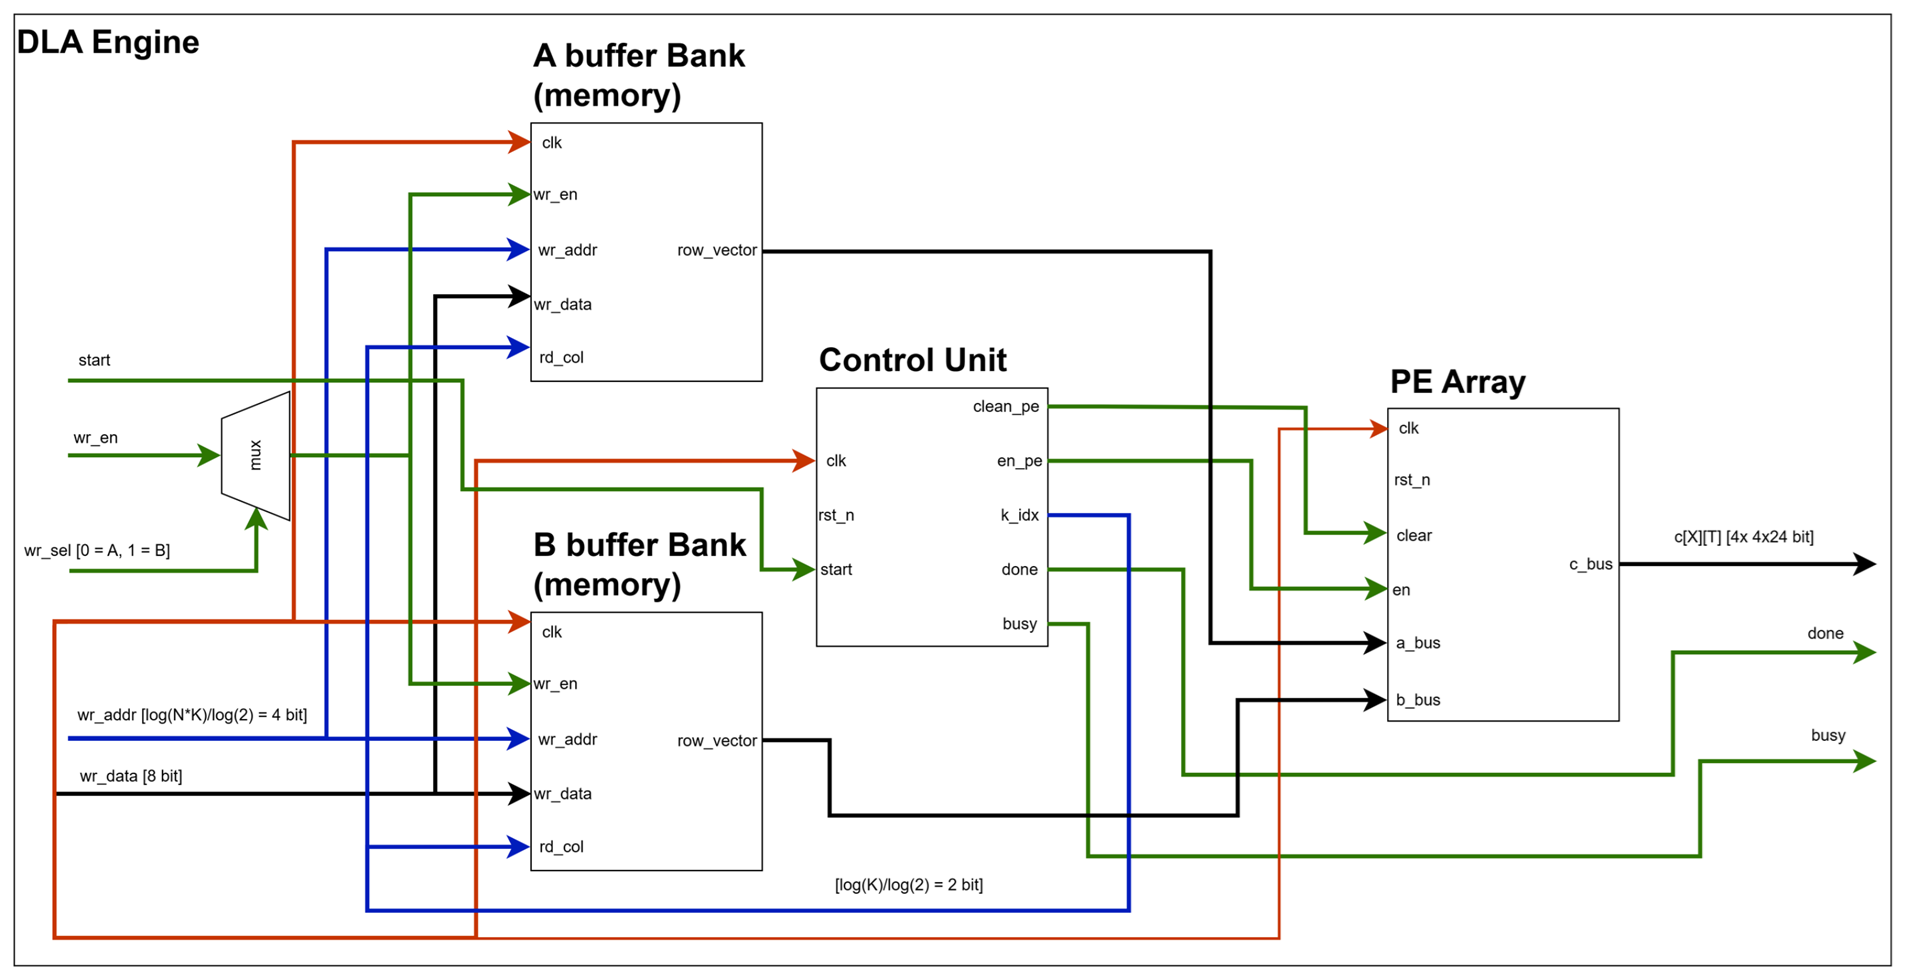
\includegraphics[width=0.75\columnwidth]{Top_level.png}
\caption{DLA engine top level.}
\label{fig:top}
\end{figure}

At the top level, shown in Fig.~\ref{fig:top}, the A buffer provides one row vector to the PE array, and the B buffer provides one column vector. The control unit generates the read index, clear signal, enable signal, done signal, and busy signal. The output bus carries the accumulated C values.

\subsection{Processing Element}

Each processing element (Fig.~\ref{fig:pe}) receives two signed 8-bit inputs. It multiplies them, sign-extends the 16-bit product to 24 bits, and adds it to a local accumulator. The accumulator is cleared at the start of each matrix multiplication. The output of each PE is one dot product.

\begin{figure}[h]
\centering
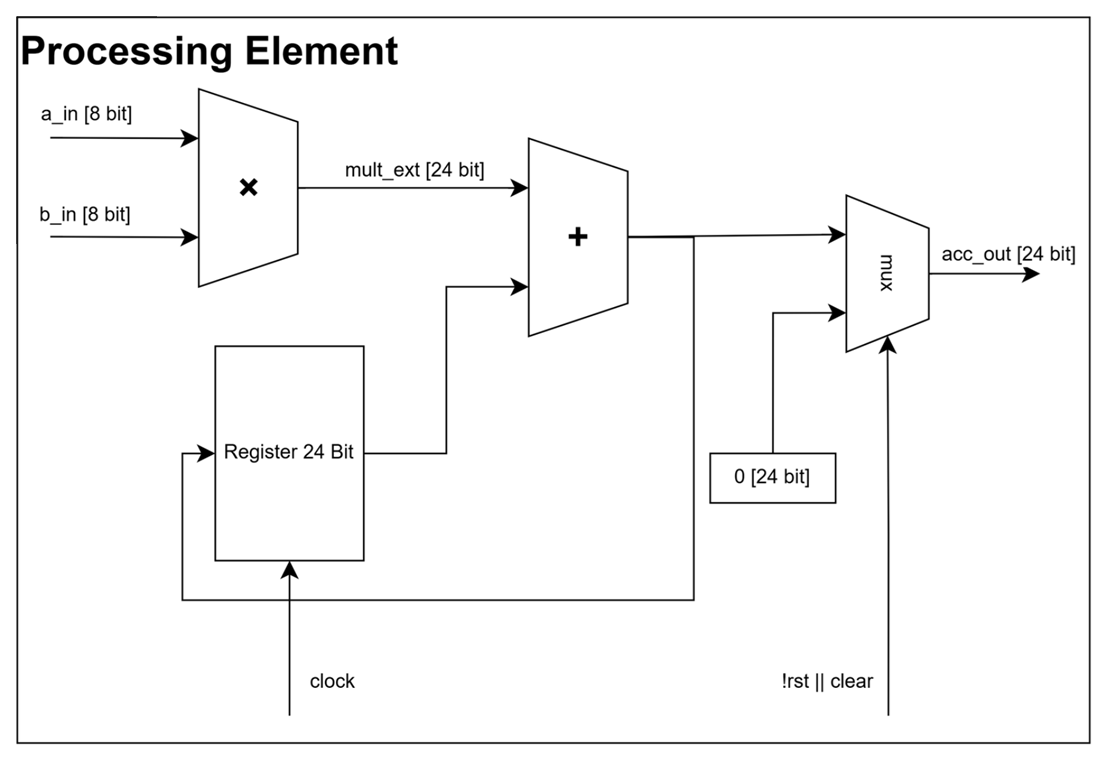
\includegraphics[width=0.72\columnwidth]{PE.png}
\caption{Processing element datapath.}
\label{fig:pe}
\end{figure}

The main computation in one PE follows
\begin{equation}
acc_{out}[n] = acc_{out}[n-1] + a_{in}[n]\,b_{in}[n].
\end{equation}
After $K$ cycles, the accumulator stores one output value of the matrix multiplication tile. A 24-bit accumulator is used so that the sum of 8-bit products has enough range for the selected layer sizes.

\subsection{PE Array}
The PE array (Fig.~\ref{fig:pearray}) instantiates 16 PEs in a $4\times4$ grid. Each row receives one activation lane, and each column receives one weight lane; the operands are broadcast along the rows and columns, and each PE accumulates its result locally (an output-stationary organization), so all 16 PEs operate in parallel and the array produces one $4\times4$ output tile after the accumulation loop finishes.

The $a\_bus$ contains four 8-bit activation values, while the $b\_bus$ contains four 8-bit weight values. The output $c\_bus$ is flattened from 16 accumulator outputs, each with 24 bits.

\begin{figure}[h]
\centering
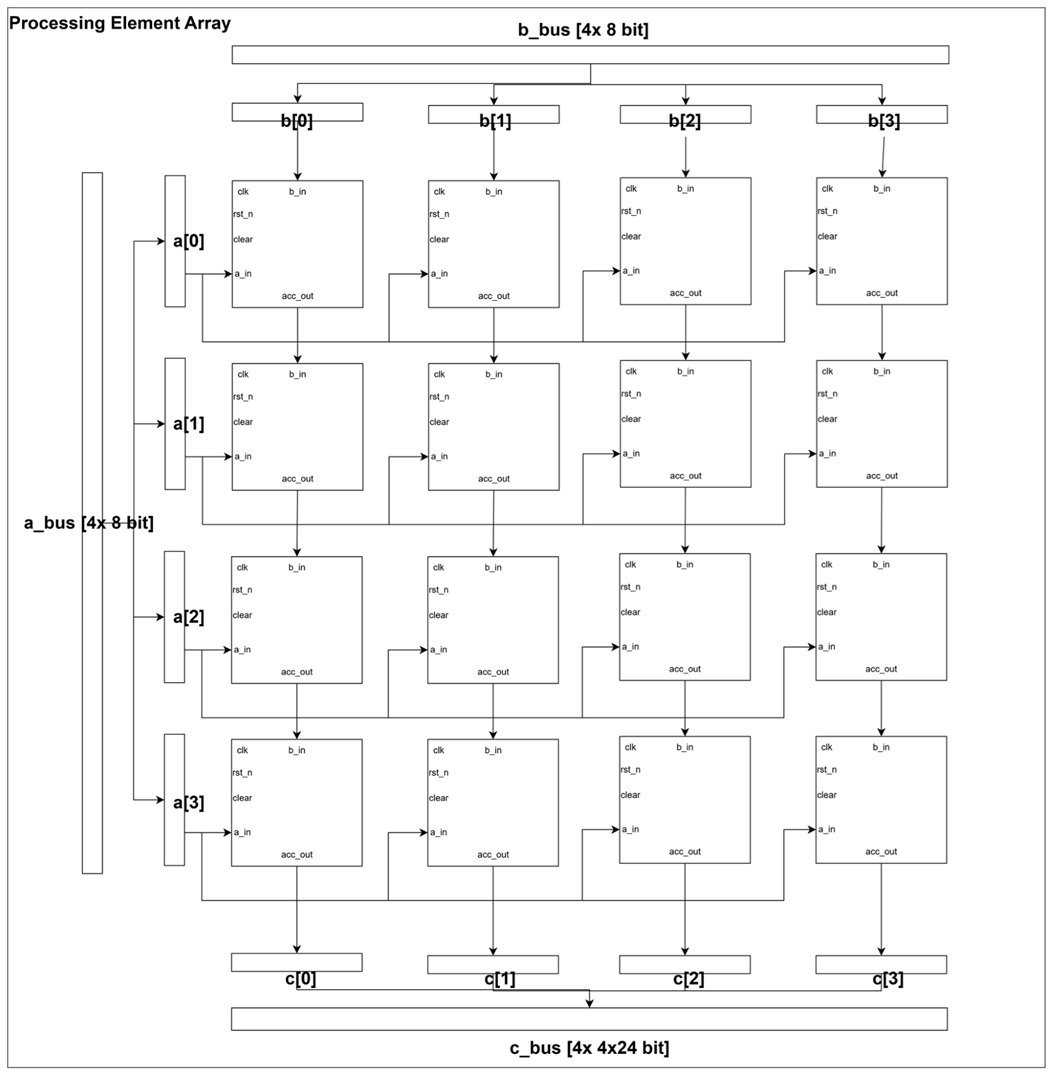
\includegraphics[width=0.8\columnwidth]{PE_Array.png}
\caption{Processing element array.}
\label{fig:pearray}
\end{figure}

\subsection{Controller FSM}
The controller uses four states (Fig.~\ref{fig:fsm}). In IDLE, it waits for START. In CLEAR, it clears all PE accumulators for one cycle. In COMPUTE, it asserts the PE-array enable and increments the A and B buffer addresses until all $K$ terms have been processed. In DONE, it raises DONE and waits for START to return low before going back to IDLE. A separate writeback sequencer then serializes the 16 accumulator values into the C buffer and raises a writeback-done flag.

\begin{figure}[h]
\centering
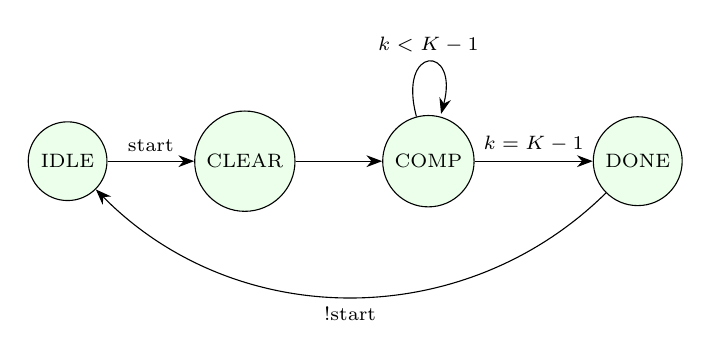
\begin{tikzpicture}[
  font=\scriptsize,>={Stealth[length=2mm]},
  st/.style={draw,circle,minimum size=10mm,fill=green!8}
]
\node[st] (idle) {IDLE};
\node[st,right=11mm of idle] (clear) {CLEAR};
\node[st,right=11mm of clear] (comp) {COMP};
\node[st,right=15mm of comp] (done) {DONE};
\draw[->] (idle) -- node[above]{start} (clear);
\draw[->] (clear) -- (comp);
\path (comp) edge[->,loop above] node{$k<K-1$} (comp);
\draw[->] (comp) -- node[above]{$k=K-1$} (done);
\draw[->] (done) to[bend left=45] node[below]{!start} (idle);
\end{tikzpicture}
\caption{Controller state machine.}
\label{fig:fsm}
\end{figure}

\subsection{SRAM Buffers}
The input and output buffers are implemented with physical $256\times8$ single-port SRAM macros. The A buffer uses four macros, one for each row lane. The B buffer also uses four macros, one for each column lane. The C buffer stores 24-bit accumulator outputs by using three 8-bit SRAM macros as byte planes of one 24-bit word. In total, the design uses eleven SRAM macros, 2{,}816 bytes of storage; the 276~KiB of INT8 generator weights are streamed through these tiles from outside rather than stored on chip. Because each tile is written to the full $K{=}256$ depth and zero-padded, the bytes actually crossing the interface per image are 331{,}776---the difference is layer L0, whose 64 inputs are padded to 256.

The SRAM wrapper has a behavioral memory model for simulation and a blackbox branch for synthesis; the power pins are not tied to logic constants in RTL but connected by the physical power delivery network during place and route. The SRAM read has one cycle of latency, so the top level delays the PE enable and completion flags by one cycle to keep data and control aligned, which prevents the PE array from accumulating invalid data after a read request.

\section{Chip-Level Integration}\label{sec:chip}

The hardened accelerator exposes 53 signal bits (a 10-bit write address alone, now that $K=256$), but the target shuttle slot provides only 20 general-purpose digital pads next to its 60 analog, 8 supply, clock, and reset pads. Instead of a pin-per-signal mapping, the chip core wraps the accelerator behind a small synchronous 4-wire serial bridge (SCLK, MOSI, CS\_N, MISO). The bridge treats SCLK as a data input: all three inputs are double-flop synchronized into the core clock domain and SCLK is edge-detected, which deliberately avoids a second clock domain. A frame is shifted MSB-first while CS\_N is low as a 2-bit command plus a 10-bit address (write frames append 8 data bits): WRITE\_A and WRITE\_B load the operand buffers, START launches one tile, and READ\_C returns one 24-bit two's-complement result on MISO. Raising CS\_N at any point aborts the frame safely. Three status flags (busy, done, writeback-done) bypass the serial link and drive pads directly, giving oscilloscope-visible liveness during board bring-up. In total the chip uses 9 of the slot's 91 pads (the serial link, the status flags, clock, and reset); the remaining bidir pads are tied off with pull-downs.

The padring is the wafer.space GF180MCU project template \cite{padring} for a $2935\times2935~\mu$m workshop slot. One consequence of the template is that the pad supply and the core supply are shorted into a single rail on every pad, so the chip is single-supply by construction. The adopted operating point is therefore 3.3~V for the whole die: the logic and SRAM are 3.3~V parts, and the foundry I/O cells are officially characterized for 3.3~V operation, so every cell on the die operates in a foundry-characterized corner and the I/O levels are directly compatible with a 3.3~V microcontroller host. Fig.~\ref{fig:chipgds} shows the final chip layout.

\begin{figure}[t]
\centering
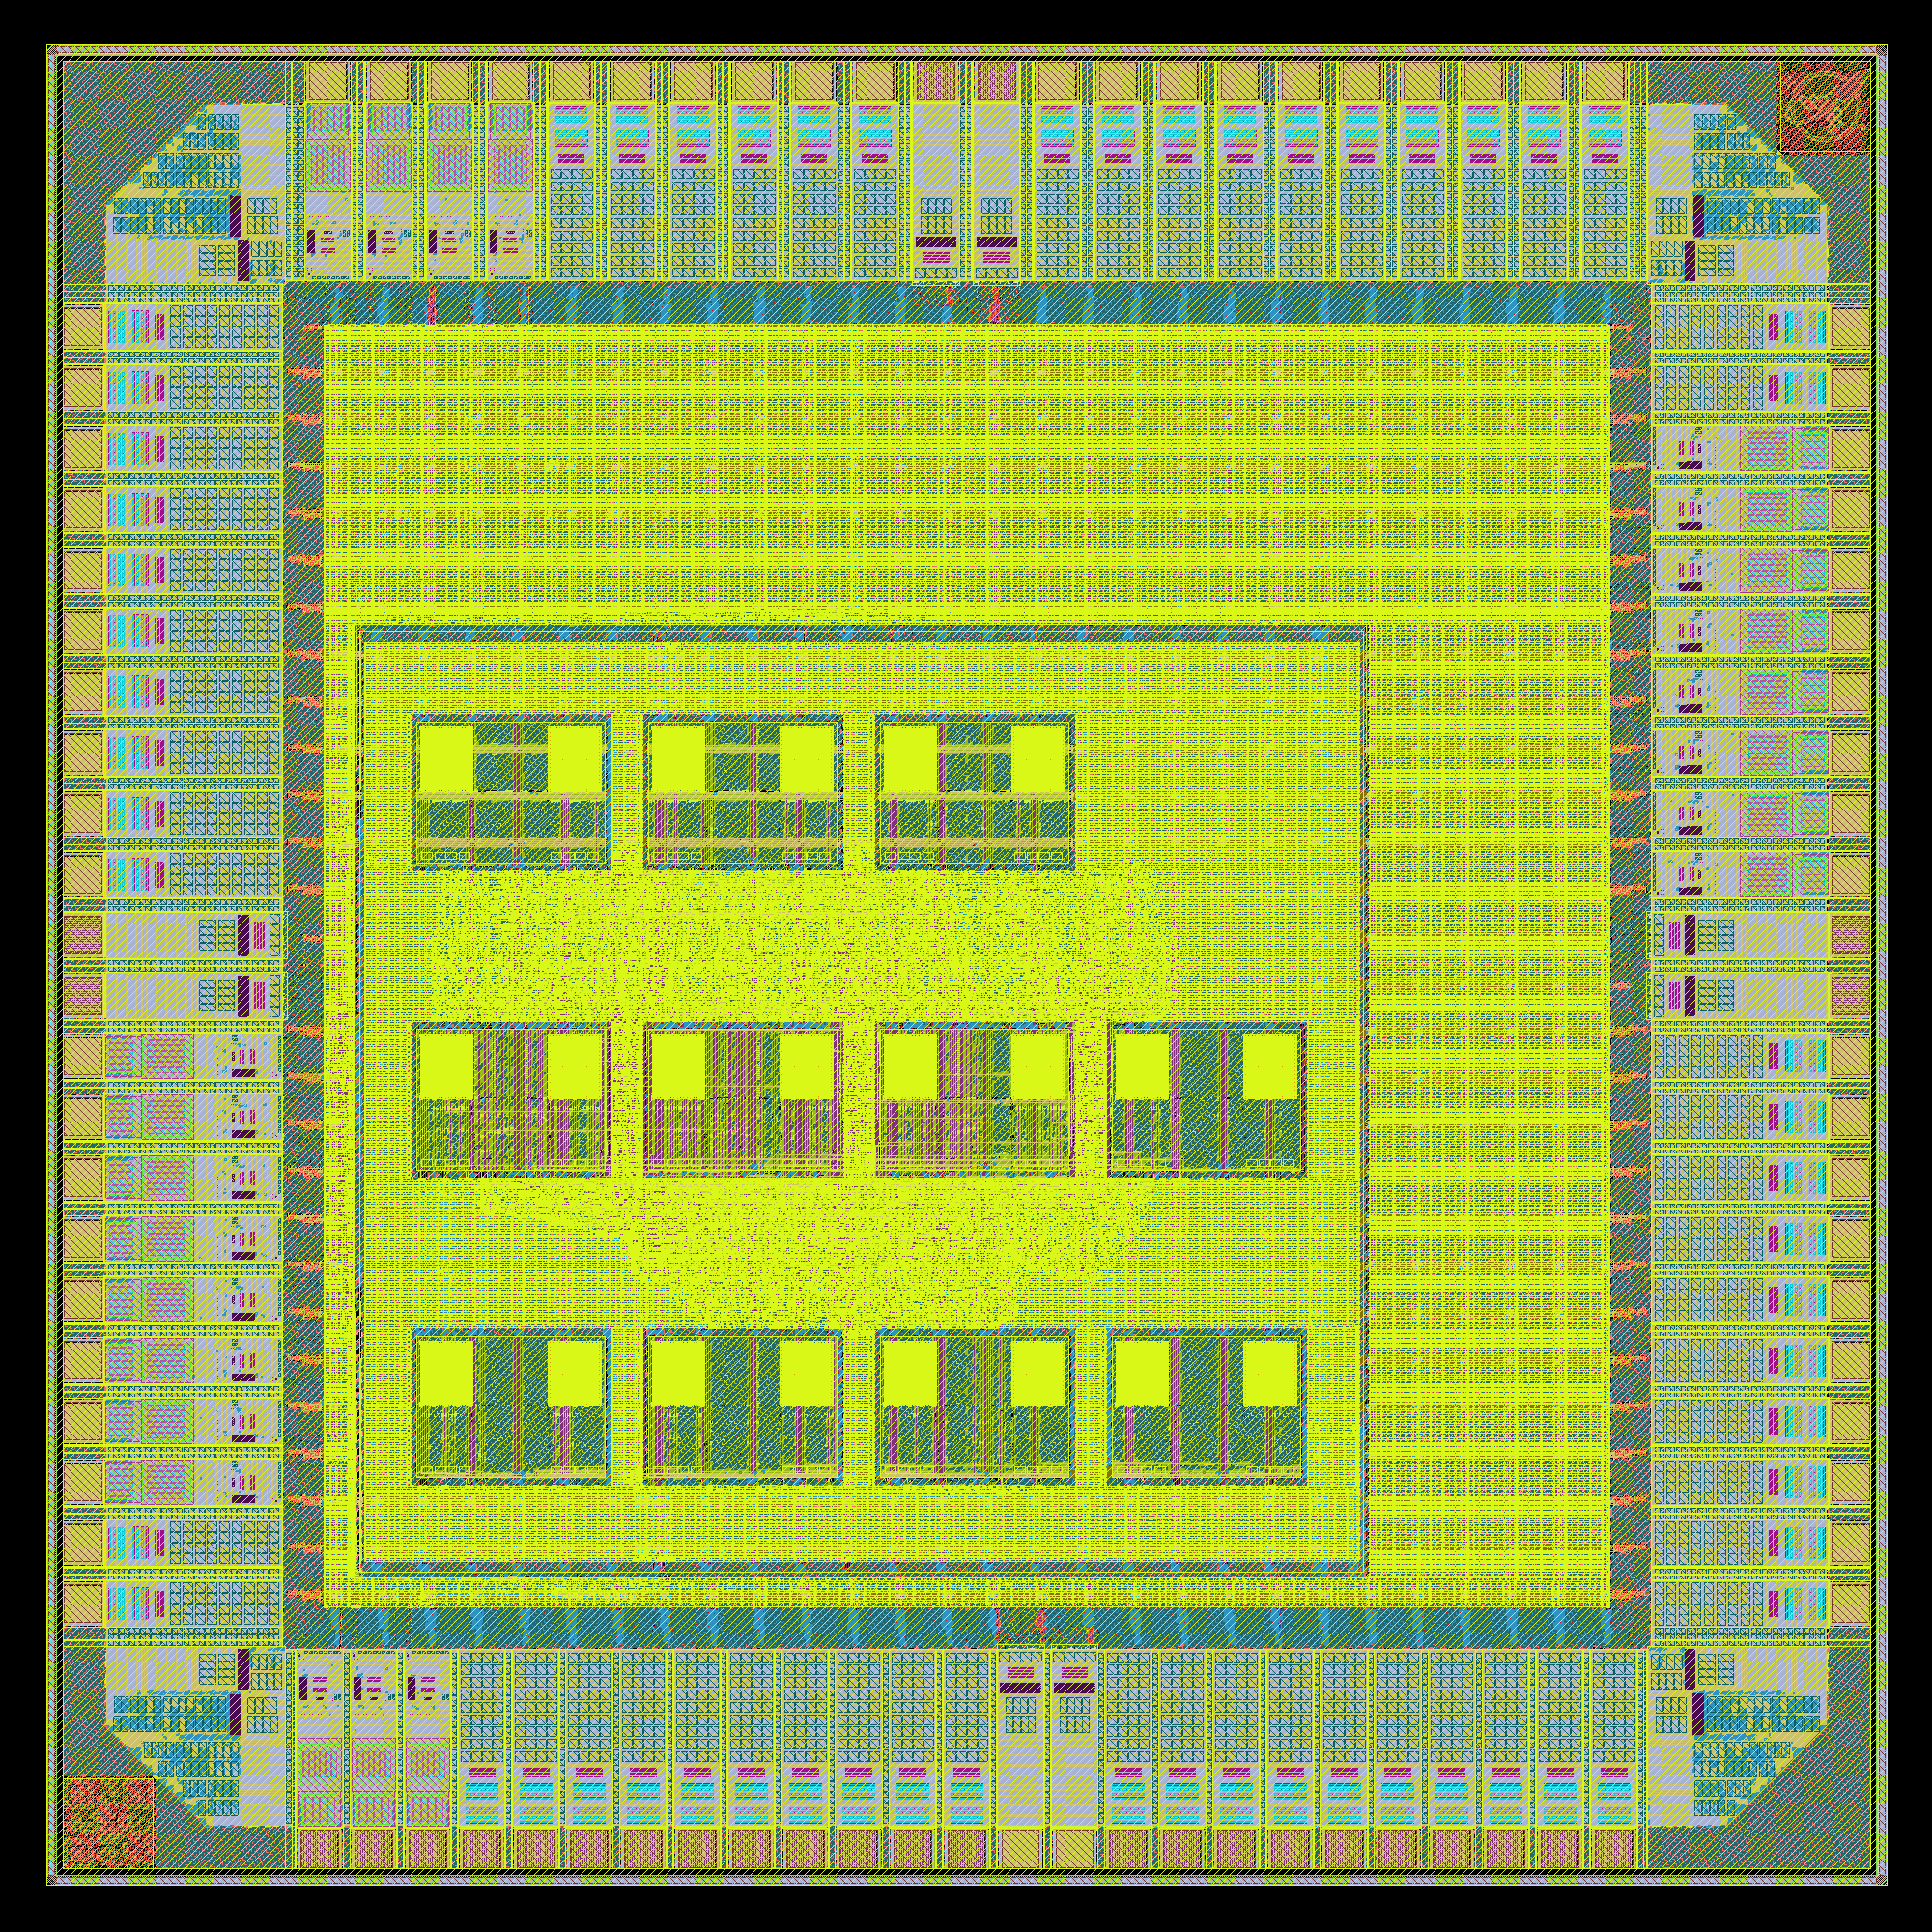
\includegraphics[width=0.60\columnwidth]{Chip_GDS.png}
\caption{Final chip layout ($2935\times2935~\mu$m slot): the DLA macro with its 11 SRAMs, the padring, and the template's identification blocks.}
\label{fig:chipgds}
\end{figure}

\section{Software to Hardware Flow}\label{sec:sw}

The system is separated into the hardware core and the verification environment. The hardware core is the DLA engine. It contains the A and B input buffers, the C output buffer, the controller, and the $4\times4$ PE array. This is the part that is hardened and taped out. The verification environment is written in Python and Verilog. It prepares quantized weights, input vectors, and reference outputs, then drives the accelerator through its normal read and write ports---or, at chip level, through the serial protocol exactly as an external host would. On the finished chip, the same role is played by a small microcontroller that streams the tile schedule over the serial link.

\begin{figure}[h]
\centering
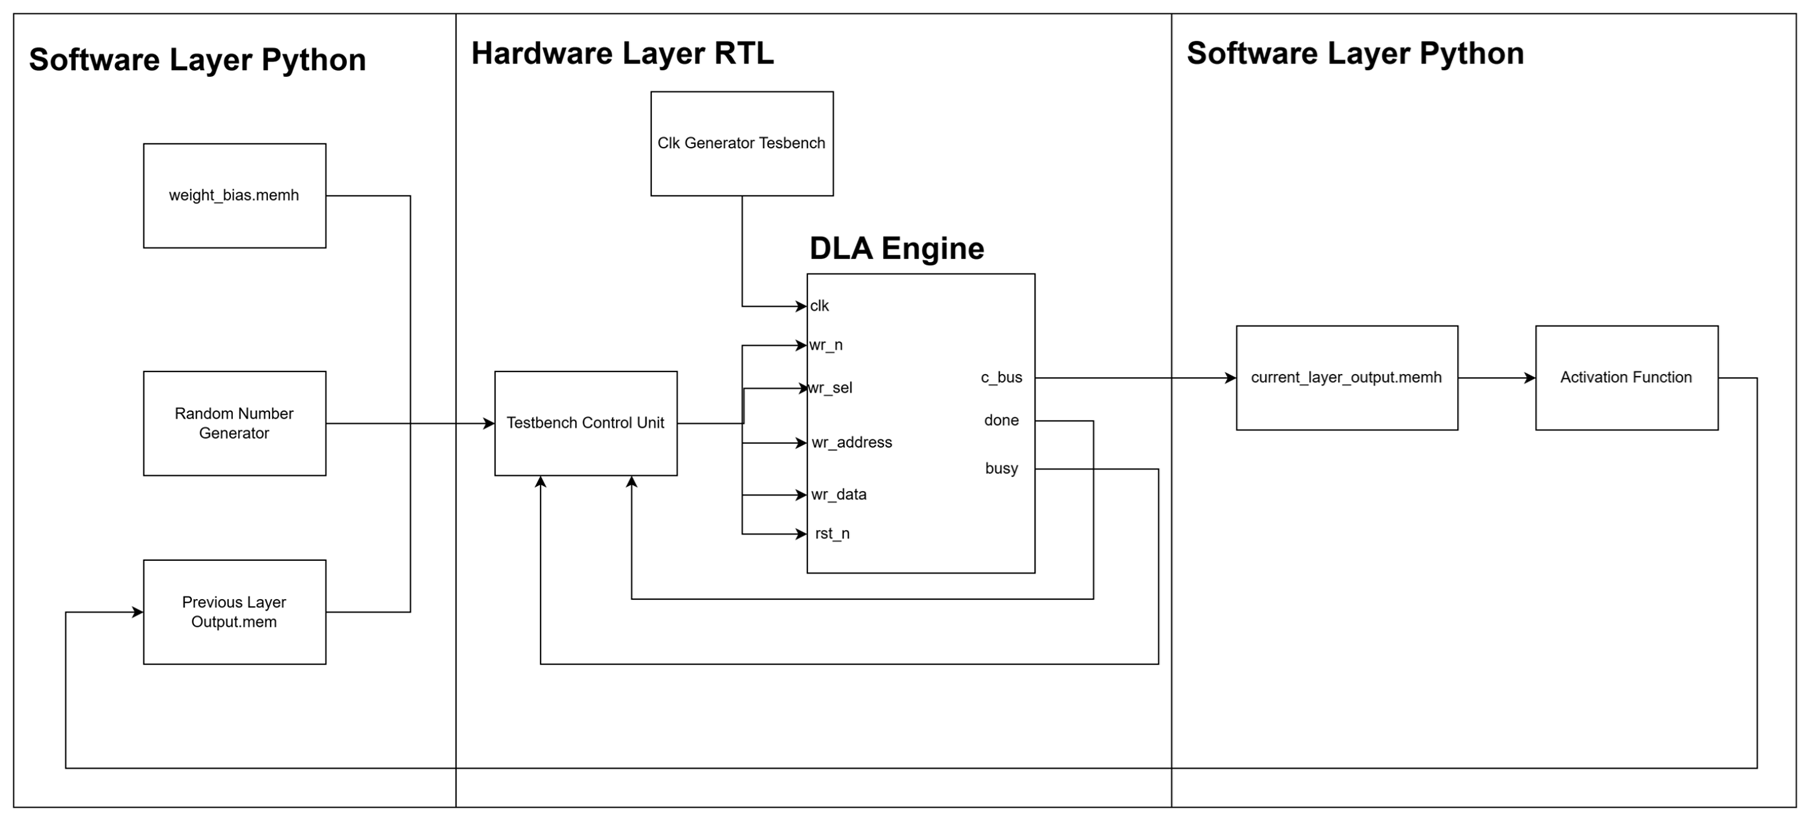
\includegraphics[width=0.62\columnwidth]{Hardware_Software_Integration.png}
\caption{Hardware and software flow.}
\label{fig:hwsoft}
\end{figure}

As shown in Fig.~\ref{fig:hwsoft}, Python prepares the input data and memory contents, then the RTL testbench loads the data into the hardware engine. After the engine finishes, the output is read back and passed to the activation-function stage. This split keeps the accelerator simple, while still allowing the complete GAN pipeline to be checked.

\subsection{Quantization and Requantization}
The original model weights are stored as 32-bit floating-point values. Before they can be used by the integer array, every weight and bias tensor is converted to signed 8-bit values using one scale factor per tensor. The scale comes from the largest absolute value in the tensor, and all scales are saved in a manifest file so the testbench can reuse the same values.

The DLA only returns the integer dot product of one tile. The rest of the math is done around it in integer form, so the hardware result matches the Python reference. For the two hidden layers, the integer result is rescaled, the bias is added, and a ReLU activation is applied before the value is quantized again to 8 bits for the next layer. For the output layer, the result is turned into a fixed-point value, passed through a tanh lookup table, and then mapped to a grayscale pixel. The lookup table is used so that tanh does not have to be computed directly in hardware.

\subsection{Choice of operand width}\label{sec:width}
INT8 was not assumed: it is the knee of a measured three-way trade-off, shown in Table~\ref{tab:quant}. The FP32 checkpoint was re-quantized to $W$ bits---weights and activations together---and the digit re-rendered through the bit-exact model, scoring the mean absolute gray-level error against the FP32 generator; the same $4\times4$ PE array RTL was then synthesized at \texttt{DATA\_W}~$=W$ against the 3.3~V standard-cell library to obtain its silicon cost.

Accuracy collapses below eight bits and saturates above it. INT4 is $16.8\times$ worse than INT8 (31.96 versus 1.90 gray levels of 255) for a $2.5\times$ smaller array, and it does not even reduce the traffic that dominates run time, because the SRAM macros are $\times 8$ and a sub-byte operand still occupies a byte unless packing logic is added. In the other direction, INT16 recovers only 0.98 gray levels---0.4\% of full scale, below the visible threshold for this workload---while nearly tripling the PE array area and doubling the weight bytes, which doubles the term that is 99\% of end-to-end latency (Section~\ref{sec:disc}). The accumulator width follows the operand width as $2W+\log_2 K$, so it also sets the C-buffer macro count: 24~bits and three byte-planes at INT8, but 40~bits and five macros at INT16.

FP16 was measured the same way rather than argued about. Because it is a different datapath rather than a parameter change, a dedicated FP16-multiply / FP32-accumulate element was written and verified bit-exact against a reference model over 8{,}192 multiply--accumulate steps before its area was quoted; FP32 accumulation is what an FP16 array needs to hold a 256-deep dot product without losing the smallest terms. It costs $2.90\times$ the INT8 array, and that figure is a floor: the unit flushes subnormals and implements no NaN or infinity handling at all, both of which a production design must add.

The instructive part is that FP16 lands essentially on top of INT16 ($2.90\times$ versus $2.96\times$) despite multiplying only $11\times11$ mantissa bits against INT16's $16\times16$. The saving in the multiplier is consumed by the alignment shifter, the leading-zero counter and the rounding logic that fixed-point arithmetic does not need. Floating point therefore buys near-exact arithmetic at both the area cost of INT16 and, needing two bytes per operand, the same doubled link time---to remove an error that Table~\ref{tab:quant} shows is already under one gray level. The dynamic range that motivates floating point is in any case handled here by the per-tensor scale together with the Q4.12 requantization, the measured saturation counters confirm the integer path is not clipping where it matters, and the open PDK provides no floating-point macro.

% generated by scripts/quant_tradeoff_study.py -- do not edit by hand
\begin{table}[h]
\caption{Operand-width trade-off. Accuracy is the mean absolute gray-level error of the rendered $28\times28$ digit against the FP32 generator; PE array area is Yosys cell area for the 16-PE array in the 3.3~V library; link time is the weight-streaming term that dominates end-to-end latency.}
\label{tab:quant}
\centering
\renewcommand{\arraystretch}{1.08}
\begin{tabular}{@{}crrrr@{}}
\toprule
Width & Mean err. & Max err. & PE area ($\mu$m$^2$) & Link time \\
\midrule
INT4 & 31.96 & 254 & 100,108 & 0.90~s \\
\textbf{INT8} & \textbf{1.90} & \textbf{46} & \textbf{252,540} & \textbf{0.90~s} \\
INT16 & 0.92 & 7 & 747,110 & 1.81~s \\
FP16$^\dagger$ & \textless 0.01 & --- & 732,407 & 1.81~s \\
\bottomrule
\end{tabular}
\\[2pt]\footnotesize $^\dagger$FP16 multiply with FP32 accumulate (\texttt{study/fp16\_mac.v}), subnormals flushed and no NaN/Inf handling: a floor on a production unit.
\end{table}


\section{Verification}\label{sec:map}

To verify the GAN RTL result, the generator is mapped onto the DLA as a sequence of tiled dense layers. For each tile, four output neurons are computed at the same time: the four weight rows are written to the A buffer bank, and the shared input vector is written into the B buffer. The DLA then performs the dot products and stores the results in the C buffer. Layer L0 uses the 64-dimensional latent vector as input, and layers L2 and L4 use the 256-dimensional activations of the previous layer; since the array has four output lanes, L0 and L2 each require 64 tiles, while L4 requires 196 tiles. The same datapath is reused for all layers.

\begin{table}[h]
\caption{Verification results.}
\label{tab:verif}
\centering
\renewcommand{\arraystretch}{1.08}
\begin{tabular}{@{}lll@{}}
\toprule
Testbench & Check & Result \\
\midrule
\texttt{d3004\_tb} & one GEMM, single lane & PASS \\
\texttt{d3004n4\_tb} & full $N{=}4$/$K{=}256$ tile, all A/B macros & PASS \\
\texttt{g3005\_tb} & one layer row & PASS \\
\texttt{g300\_pipeline\_tb} & full 784-pixel image & PASS \\
\texttt{chip\_core\_dla\_tb} & pad-level serial protocol & PASS \\
gate-level (unit) & routed netlist, $N{=}4$/$K{=}256$ vectors & PASS \\
gate-level (image) & routed netlist, full 784-pixel image & PASS \\
\bottomrule
\end{tabular}
\end{table}

Table~\ref{tab:verif} summarizes the verification stack; all testbenches check against Python golden vectors. The two gate-level runs re-simulate the actual routed netlist produced by the physical flow (including its inserted buffers and roughly 7{,}700 antenna diodes) with the behavioral SRAM model and reproduce the golden results bit-exactly, closing the gap between ``the RTL is correct'' and ``the taped-out netlist is correct.'' The stack caught two real integration bugs before sign-off: the A and B buffers use different write-address layouts (row-major versus $k$-major), which one testbench initially got wrong, and the serial READ\_C path needed an extra wait state because a C-buffer address update is not visible to the registered SRAM read until the next cycle.

\begin{figure}[h]
\centering

\includegraphics[width=0.19\linewidth]{digit_seed6.jpg}\hspace{4mm}

\includegraphics[width=0.19\linewidth]{digit_seed5.jpg}\hspace{4mm}
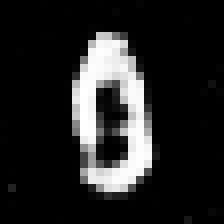
\includegraphics[width=0.19\linewidth]{digit_seed9.jpg}
\caption{Generated digit samples.}
\label{fig:samples}
\end{figure}

Fig.~\ref{fig:samples} shows examples of generated $28\times28$ images. The visual quality is limited by the small generator and by INT8 quantization, but the images are enough to verify that the full software-to-hardware path is running.

\section{Physical Implementation}\label{sec:phys}

The design is implemented with LibreLane \cite{librelane} on the GF180MCU open PDK \cite{gf180pdk} in two stages: the accelerator is hardened as a macro, and the macro GDS/LEF/liberty views are then consumed by the padring integration.

\subsection{Single-Supply 3.3~V Library Migration}
The buffer SRAM macro \cite{gf180sram} is a 3.3~V IP, but the open PDK ships only 5~V digital standard cells, so a first version of this design mixed a 5~V core with 3.3~V SRAMs---workable for layout checks but requiring level shifting on real silicon. The design was therefore migrated to the third-party \texttt{gf180mcu\_as\_sc\_mcu7t3v3} native-3.3~V standard-cell library, which ships nine liberty corners and a LibreLane integration, making the whole die single-supply. Bringing the library up surfaced three real bugs in its flow integration (a missing timing-corner variable, a synthesis-exclusion filename mismatch, and non-synthesizable \texttt{\$random} initializers in six sequential-cell models that crashed lint); all were fixed at the library source. The 3.3~V cells proved much faster than the 5~V ones: the initial run at the old 75~ns clock closed with $+44$~ns of setup slack, so the clock was retimed to 40~ns (25~MHz), and the SRAM liberty corners now match the standard cells one-to-one at every PVT point.

\subsection{Hardening the Accelerator Macro}
A few configuration points were essential. A synthesis define keeps the SRAM as a hard macro---without it, the memory is silently built from flip-flops. The eleven macros are registered with their LEF/GDS/liberty views and placed explicitly on a $4\times3$ grid with routing channels. The SRAM power pins only reach Metal3, so the macro power-grid connection had to be made on Metal3 instead of the default higher layers. Routing was allowed up to Metal5, standard-cell padding was added for diode pin access, and antenna diodes are inserted heuristically at placement time with the in-router antenna repair disabled.

The antenna check required an empirical closure method. Direct in-router antenna repair aborts unreliably in this flow because its verification reroute fails pin access on already-placed clock-net diodes, and the remaining violation was a wire-length problem on a long buffered net that already carried several diodes, so adding more diodes could not help. Larger floorplan changes (macro clustering, row swaps, fanout caps) consistently made the antenna count worse by creating new long routes. What worked---both for the earlier 5~V version and again here---is a small deterministic perturbation of the placement density on the same floorplan, which re-rolls which nets route long. Table~\ref{tab:antenna} shows the sweep for the final $K{=}256$ netlist: density 63 reaches zero antenna violations, and re-running that configuration reproduces a byte-identical placement-and-routing database, so the result is deterministic rather than a routing fluke.

\begin{table}[h]
\caption{Antenna closure sweep (placement density, $K{=}256$ netlist, 40~ns clock). All runs are DRC-, LVS-, and timing-clean.}
\label{tab:antenna}
\centering
\renewcommand{\arraystretch}{1.08}
\begin{tabular}{@{}lccl@{}}
\toprule
Density (\%) & Antenna nets & Setup slack (ns) & Result \\
\midrule
61 & 2 & $+15.53$ & \\
60 & 5 & $+15.75$ & worse \\
62 & 1 & $+15.60$ & \\
63 & 0 & $+15.12$ & clean sign-off \\
63 (re-run) & 0 & $+15.12$ & identical DEF \\
\bottomrule
\end{tabular}
\end{table}

\begin{figure}[t]
\centering
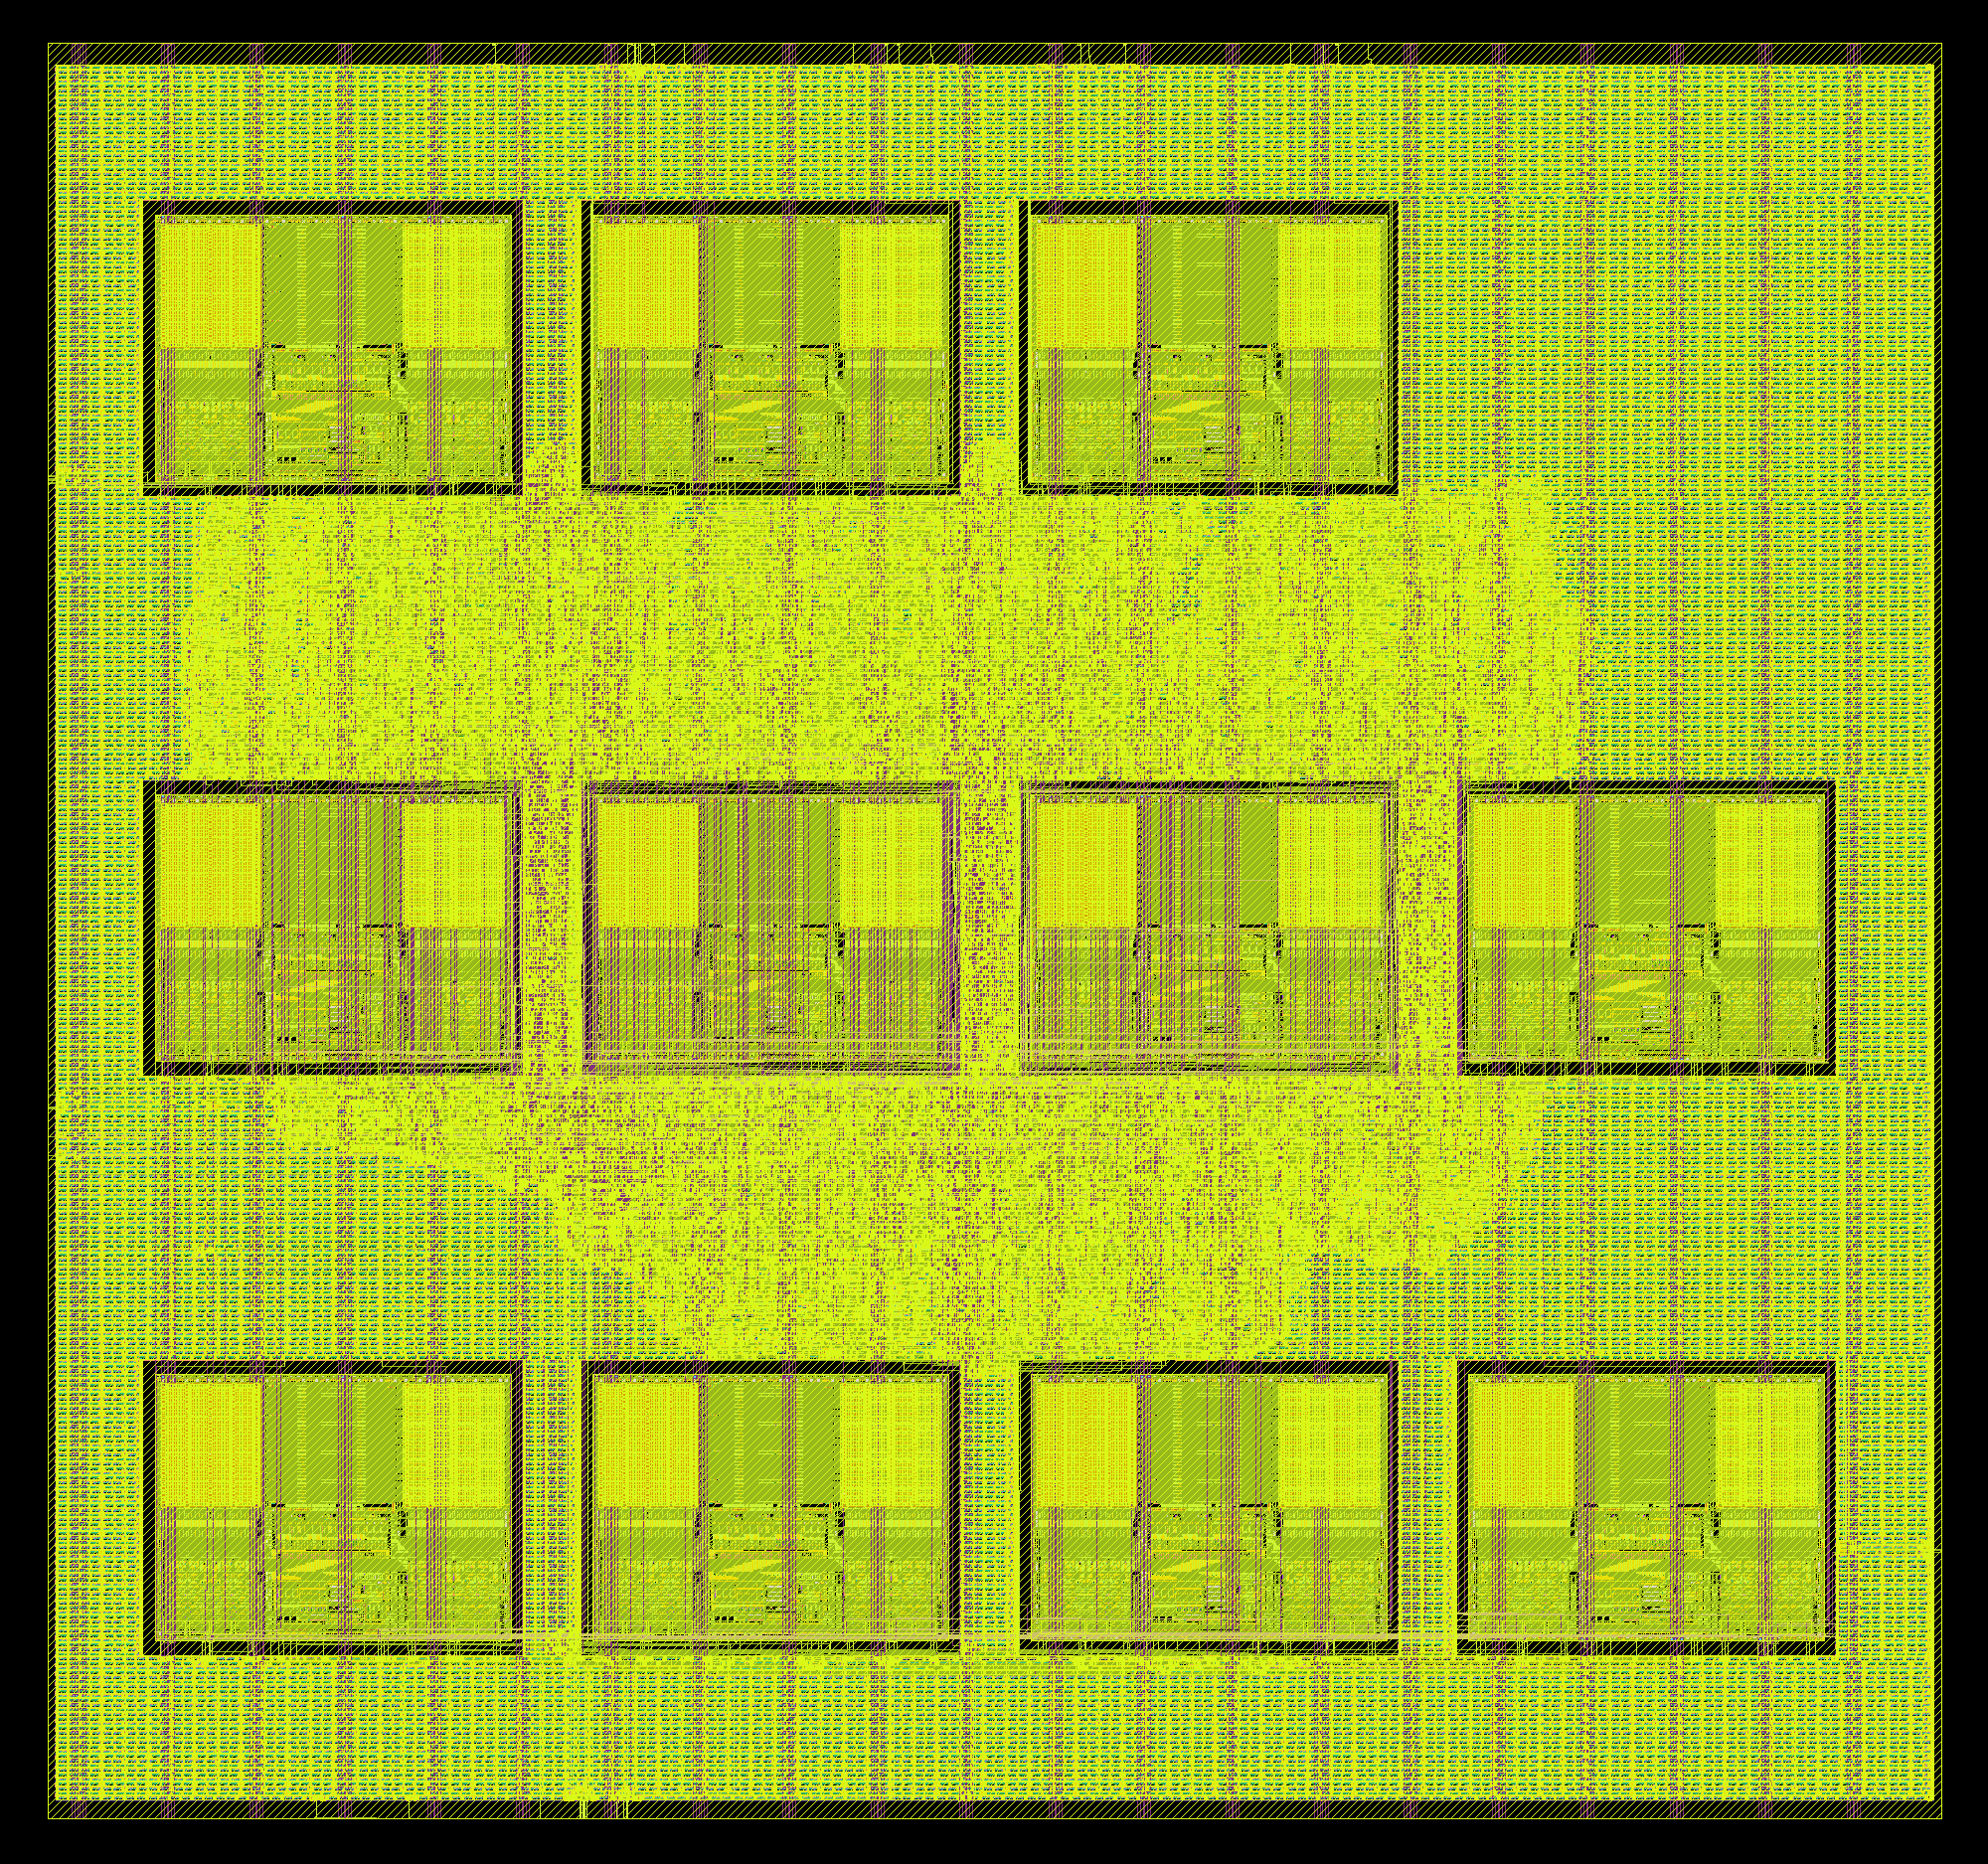
\includegraphics[width=0.63\columnwidth]{Stage1_GDS.png}
\caption{Hardened accelerator macro ($1600\times1500~\mu$m) with the eleven SRAM macros on a $4\times3$ grid.}
\label{fig:layout}
\end{figure}

Fig.~\ref{fig:layout} shows the resulting macro layout, and Table~\ref{tab:signoff} summarizes the sign-off results. Magic reports zero DRC errors, Netgen reports zero LVS errors, and the antenna report has zero violating nets and pins. The design meets the 40~ns clock at all nine STA corners: the worst setup slacks per corner family are $+23.41$~ns (TT), $+15.12$~ns (SS, 125\,\textdegree C, 3.0~V), and $+26.54$~ns (FF), and the worst hold slacks are $+0.260$, $+0.333$, and $+0.150$~ns respectively. The reported nominal power is 162~mW, almost entirely internal power estimated with the flow's default switching activity, and should be read as a conservative tool estimate rather than a measurement.

\begin{table}[h]
\caption{Hardened macro results.}
\label{tab:signoff}
\centering
\renewcommand{\arraystretch}{1.08}
\begin{tabular}{@{}ll@{}}
\toprule
Metric & Value \\
\midrule
Process & GF180MCU, 180 nm \\
Standard cells & \texttt{gf180mcu\_as\_sc\_mcu7t3v3} (3.3 V) \\
Die area & $1600\times1500~\mu$m \\
Core area & 2.326 mm$^2$ \\
Utilization & 48.6\% \\
SRAM macros & 11 \\
Standard-cell instances & 31,711 \\
Sequential cells & 406 \\
Clock period & 40 ns (25 MHz) \\
Worst setup slack (9 corners) & $+15.12$ ns \\
Worst hold slack (9 corners) & $+0.150$ ns \\
Magic DRC / Netgen LVS & 0 / 0 errors \\
Antenna & 0 nets, 0 pins \\
Power (nominal, tool estimate) & 162 mW \\
\bottomrule
\end{tabular}
\end{table}

\subsection{Full-Chip Implementation}
The padring integration re-runs the complete flow with the hardened macro as a black box. Two macro-interface issues had to be resolved: the macro's behavioral SRAM wrapper had to be black-boxed for the chip-level static timing reader, and four short power-strap fragments that the macro LEF exports as pins lie entirely under a Metal5 routing obstruction, which the chip-level power-grid builder rejects; they were reclassified as obstructions, which is electrically equivalent and strictly more conservative.

Chip-level timing needed particular care. The first sign-off run reported infinite slack at every corner---a hollow result: with no pad liberty views loaded, the timing tool treated every pad as an empty black box, the clock defined on the clock pad's output degraded to a virtual clock, and nothing was actually constrained. The fix was to load the foundry pad liberty at its 3.3~V characterization corners. The now-real numbers exposed one more constraint bug: the template's blanket input delays imposed hold checks on the three asynchronous serial inputs, which are synchronizer-guarded by design, and these were replaced by false-path constraints. After both fixes, all nine corners close with real paths (Table~\ref{tab:chip}).

\begin{table}[h]
\caption{Full-chip sign-off results.}
\label{tab:chip}
\centering
\renewcommand{\arraystretch}{1.08}
\begin{tabular}{@{}ll@{}}
\toprule
Metric & Value \\
\midrule
Slot die & $2935\times2935~\mu$m \\
Pads & 91 (9 used) \\
Instances / macros & 71,668 / 3 \\
Magic DRC / KLayout DRC & 0 / 0 \\
Chip-level LVS & 0 errors \\
Antenna & 0 nets, 0 pins \\
GDS XOR (Magic vs.\ KLayout) & 0 \\
Worst setup slack (9 corners) & $+21.67$ ns \\
Worst hold slack (9 corners) & $+0.329$ ns \\
Worst IR drop & 0.31 mV \\
\bottomrule
\end{tabular}
\end{table}

\subsection{Comparison}
Table~\ref{tab:compare} places this work against representative MAC-array accelerators spanning three orders of magnitude in scale: the datacenter-class TPU~v1 \cite{tpu}, the mobile CNN accelerator Eyeriss \cite{eyeriss}, and the small embedded design of Wang et al. \cite{wang} that is closest in array size. Absolute area and power are not comparable across such different nodes, so normalized figures are given alongside: peak throughput per unit area and per watt, both of which are process-sensitive but at least scale-invariant.

Our design occupies 2.326~mm$^2$ of core area and dissipates 162~mW at 25~MHz, giving 0.344~GOPS/mm$^2$ and 4.95~GOPS/W. It is comfortably the least efficient entry, and the gap is not marginal: Wang et al. reach roughly $115\times$ our GOPS/W. Three factors account for almost all of it, and none is architectural. The process is $4.5\times$ coarser in feature size, worth roughly two orders of magnitude in energy per operation on its own; the clock is deliberately conservative at 25~MHz where the comparison designs run in the hundreds of megahertz; and the array is 16 MACs against their 8 operating at far higher utilization. Under ideal $(L/L_0)^2$ scaling our core would be 0.115~mm$^2$ at 40~nm, which is the fairer basis for an area reading, though such scaling is optimistic for an SRAM-dominated design---eleven macros account for a large share of the area here---and should be treated as a bound rather than a projection.

The claim of this work is therefore not efficiency but reproducibility on an open process. The entire result, from the quantization scripts to the final chip GDS with DRC, LVS, antenna and nine-corner timing sign-off, is produced by a public open-source flow on an open PDK, which none of the compared designs offer; the closed 40~nm and 28~nm results cannot be re-derived, re-targeted or corrected by a reader. For a shared-shuttle educational tapeout that property is the point, and the efficiency figures above are best read as the price of it.

% ---------------------------------------------------------------------------
% AUTHORS: the two leftmost data columns must be completed from the source
% papers before submission -- the values were deliberately NOT filled in here
% because they cannot be verified from this repository.  Fields needed per work:
%   technology node, array size and dataflow, arithmetic precision, core area,
%   power and the clock/operating point it was measured at, peak throughput.
% Then compute GOPS/mm^2 and GOPS/W the same way as the "This work" column
% (peak GOPS divided by core area / total power).  Suggested primary sources:
%   TPU v1  -- Jouppi et al., ISCA 2017, Table 2 / Fig. 2 (28 nm, 65,536 MACs)
%   Eyeriss -- Chen et al., IEEE JSSC 52(1), 2017 (65 nm, 168 PEs)
% If a number is unavailable in the source, print "n/r" rather than estimating.
% ---------------------------------------------------------------------------
\begin{table}[h]
\caption{Comparison with representative MAC-array accelerators. Normalized figures use peak throughput over core area and total power.}
\label{tab:compare}
\centering
\resizebox{\columnwidth}{!}{%
\renewcommand{\arraystretch}{1.08}
\begin{tabular}{@{}lcccc@{}}
\toprule
Parameter & TPU v1 \cite{tpu} & Eyeriss \cite{eyeriss} & Wang \cite{wang} & This work \\
\midrule
Technology        & 28 nm  & 65 nm  & 40 nm                     & GF180MCU 180 nm \\
Array             & $256^2$ & 168 PE & $2\times2\times2$        & $4\times4$, $K{=}256$ \\
Precision         & INT8   & INT16  & \dots                     & INT8 \\
Core area (mm$^2$)& \dots  & \dots  & 11.97                     & 2.326 \\
Power             & \dots  & \dots  & 96.35 mW                  & 162 mW \\
Peak throughput   & \dots  & \dots  & 54.61 GOPS                & 0.8 GOPS \\
GOPS/mm$^2$       & \dots  & \dots  & 4.56                      & 0.344 \\
GOPS/W            & \dots  & \dots  & 566.8                     & 4.95 \\
Open-source flow  & No     & No     & No                        & Yes \\
\bottomrule
\end{tabular}}
\end{table}

\section{Discussion}\label{sec:disc}
The array performs 16 MAC operations per cycle, a peak of 0.8~GOPS at 25~MHz. Table~\ref{tab:latency} breaks one image down by stage. The per-tile cost is measured rather than assumed: a dedicated testbench reports 278 cycles from \texttt{start} to \texttt{wb\_done}, of which 256 are the $K$ accumulation and 22 are controller sequencing plus the serialized writeback of the sixteen accumulators. Across the 324 tiles of the three layers---64 for L0, 64 for L2 and 196 for L4---that is 90{,}072 cycles, or 3.60~ms of array time at 40~ns. Effective utilization is lower still, because the broadcast schedule computes only four unique neurons per tile.

That compute time is not, however, the latency a user sees. Streaming the weights across the 4-wire link costs one 20-edge frame per byte, and with the serial clock at \texttt{clk}/8---one edge every four core clocks, or 160~ns---the 331{,}776 weight bytes of a single image take 1.06~s. Adding the input vectors, the \texttt{START} commands and the C read-back gives \textbf{1.076~s end to end per image}, of which the PE array is busy for 0.33\%: the link is $298\times$ the compute. Effective throughput is 0.93 images/s, or 0.62~MOPS against the 0.8~GOPS peak.

This is a property of the workload, not an implementation defect. A matrix--\emph{vector} product reuses no weight, so 1.01~weight bytes must cross the link per MAC and no achievable on-chip SRAM changes that; with 538~KiB of model against 2.8~KiB of buffer, the host is necessarily inside the inner loop. The consequences are worth stating plainly for anyone reproducing this class of design: peak GOPS is close to meaningless here, and the useful levers are all on the data-movement side. Widening the host interface is the largest: an 8-bit parallel write bus reduces the cost from 20 edges per byte to about one, and batching several latents against one weight stream amortizes the dominant term directly. Both were implemented and measured on a follow-on variant of this design, which reaches 58--62$\times$ end-to-end over the baseline serial link by combining the two. Weight-stationary reuse, double buffering, or a compressed weight format would attack the same term.

% generated by scripts/analyze_latency.py -- do not edit by hand
\begin{table}[h]
\caption{End-to-end latency breakdown for one $28\times28$ image (40~ns clock, serial clock at \texttt{clk}/8).}
\label{tab:latency}
\centering
\renewcommand{\arraystretch}{1.08}
\begin{tabular}{@{}lrrr@{}}
\toprule
Stage & Bytes & SCLK edges & Time \\
\midrule
weight stream (A) & 331,776 & 6,635,520 & 1.593 s \\
input vector (B) & 768 & 15,360 & 3.686 ms \\
START commands & --- & 3,888 & 933.120 us \\
result read (C) & 3,888 & 46,656 & 11.197 ms \\
\midrule
Serial link total & --- & 6,701,424 & 1.608 s \\
PE array compute & --- & --- & 3.603 ms \\
\midrule
\textbf{End to end} & --- & --- & \textbf{1.612 s} \\
\bottomrule
\end{tabular}
\end{table}


The implementation also shows a trade-off between timing and antenna closure: floorplans that shortened the SRAM-to-MAC critical path consistently increased the antenna count, and the priority here was a clean physical sign-off rather than the fastest possible clock. The earlier voltage-domain concern was resolved structurally---the padring shorts the pad and core supplies, so the single-supply 3.3~V operating point removes the level-shifting problem entirely, at the cost of 3.3~V (rather than 5~V) I/O levels, which matches the intended microcontroller host anyway. A true dual-rail variant was evaluated and deferred because the only available dual-voltage pad library is not yet silicon-ready. A bring-up plan for the returned silicon is prepared: current-limited power-on, status-pin checks, replay of the unit-test golden vectors over the serial link from a bit-banging 3.3~V microcontroller, and finally a full streamed digit render.

\section{Conclusion}\label{sec:concl}
This work implements a small INT8 GAN-generator accelerator on GF180MCU and carries it to a tapeout-ready chip with a fully open-source flow. The design replaces behavioral memory arrays with eleven SRAM macros, uses a $4\times4$ PE array with a native $K{=}256$ accumulation depth for tiled matrix multiplication, and verifies the output against Python references at every level up to a bit-exact full-image render on the routed post-layout netlist. Both the hardened macro and the integrated chip pass DRC, LVS, and antenna checks cleanly and close timing at 40~ns across nine corners on a single 3.3~V supply. The main remaining work is silicon bring-up and improving data reuse for higher throughput.

\section*{Acknowledgment}
The authors thank the open-source EDA community, the GlobalFoundries open PDK program for GF180MCU and the SRAM macro, and the wafer.space chipathon program for the padring template and the shuttle slot targeted by this work.

\section*{Author Contributions}
W. Anthony: RTL architecture, PE array design, RTL-to-GDS flow, verification. I M. M. Surya W.M.: RTL architecture, MLP GAN architecture, block diagrams, verification. J. R. Saragi: GAN concept, RTL architecture, verification. F. A. Rahagi: RTL architecture, RTL-to-GDS flow. M. P. Adipratama: RTL architecture, verification, RTL-to-GDS flow, chip-level integration.

\begin{thebibliography}{12}
\bibitem{tpu} N. P. Jouppi \emph{et al.}, ``In-datacenter performance analysis of a tensor processing unit,'' in \emph{Proc. ISCA}, 2017.
\bibitem{survey} C. Silvano \emph{et al.}, ``A survey on deep learning hardware accelerators for heterogeneous HPC platforms,'' \emph{ACM Computing Surveys}, 2025.
\bibitem{eyeriss} Y.-H. Chen, T. Krishna, J. S. Emer, and V. Sze, ``Eyeriss: An energy-efficient reconfigurable accelerator for deep convolutional neural networks,'' \emph{IEEE J. Solid-State Circuits}, vol. 52, no. 1, pp. 127--138, 2017.
\bibitem{jacob} B. Jacob, S. Kligys, B. Chen, M. Zhu, M. Tang, A. Howard, H. Adam, and D. Kalenichenko, ``Quantization and training of neural networks for efficient integer-arithmetic-only inference,'' in \emph{Proc. IEEE/CVF CVPR}, 2018.
\bibitem{wang} C. C. Wang, S. H. Luo, H. C. Wu, R. G. B. Sangalang, C. P. Jou, and H. Hsia, ``A 54.61 GOPS 96.35 mW digital logic accelerator for underwater object recognition DNN using 40 nm CMOS process,'' in \emph{Proc. IEEE 6th Int. Conf. AI Circuits and Systems (AICAS)}, 2024.
\bibitem{goodfellow} I. Goodfellow, J. Pouget-Abadie, M. Mirza, B. Xu, D. Warde-Farley, S. Ozair, A. Courville, and Y. Bengio, ``Generative adversarial nets,'' in \emph{Proc. NeurIPS}, 2014.
\bibitem{ganpretrained} C. Singh, ``GAN/VAE pretrained PyTorch models,'' \url{https://github.com/csinva/gan-vae-pretrained-pytorch}.
\bibitem{dlaengine} ``DLA Engine,'' GitHub, \url{https://github.com/wlmoi/DLA_Engine}.
\bibitem{padring} wafer.space, ``GF180MCU project template,'' \url{https://github.com/wafer-space/gf180mcu-project-template}.
\bibitem{librelane} The LibreLane project, ``LibreLane: an open-source RTL-to-GDSII flow,'' \url{https://github.com/librelane/librelane}.
\bibitem{gf180pdk} GlobalFoundries and Google, ``GF180MCU open-source PDK,'' \url{https://github.com/google/gf180mcu-pdk}.
\bibitem{gf180sram} R. T. Edwards, ``GF180MCU OCD IP SRAM macros,'' \url{https://github.com/RTimothyEdwards/gf180mcu_ocd_ip_sram}.
\end{thebibliography}

\end{document}
